\chapter{Projections for the Proposed Measurements}
\label{chap:reach}

\section{Monte-Carlo Simulation}
An event generator for DVCS/BH and exclusive $\pi^0$ electroproduction on the 
neutron inside a deuterium target has been developed \cite{ahmed}. The DVCS 
amplitude is calculated according to the BKM formalism \cite{Belitsky:2001ns}, 
while the GPDs have been taken from the standard CLAS DVCS generator 
\cite{PhysRevD.60.094017,Guidal:2004nd}.  The Fermi-motion distribution is 
calculated with the Paris potential \cite{PhysRevC.21.861}.

The output of the event generator was fed through CLAS12 official simulation 
and reconstruction chain, to simulate the acceptance and resolutions of 
electrons and photons in the Forward Detector. Final state neutrons being 
detected in the central detector of CLAS12, and the final state recoiling 
protons in the BONuS12 RTPC. 

Figure~\ref{fig:el_kin} shows the kinematic distributions of the DVCS electrons 
being detected and reconstructed in the forward detector of CLAS12 spectrometer 
in terms of the energy as a function of the polar angle ($\theta$) and the 
azimuthal angle ($\phi$) as a function of $\theta$. Figure~\ref{fig:photon_kin} 
presents the kinematic distributions of the neutron-DVCS photons detected in 
the CLAS12 forward detector.



~\ref{fig:photon_kin}, and~\ref{n_th_p} show $\theta$ as a function of momentum 
in the lab frame and for, respectively, the electron, the photon and the 
neutron.  The two panels of Fig.~\ref{n_th} are one-dimensional plots, showing, 
respectively, the momentum and the polar angle of the recoil neutron.  As 
expected, the electron and the photon are mostly emitted at forward angles, 
while the recoil neutron is going at backwards angles.

\begin{figure}[htb]
\centering
   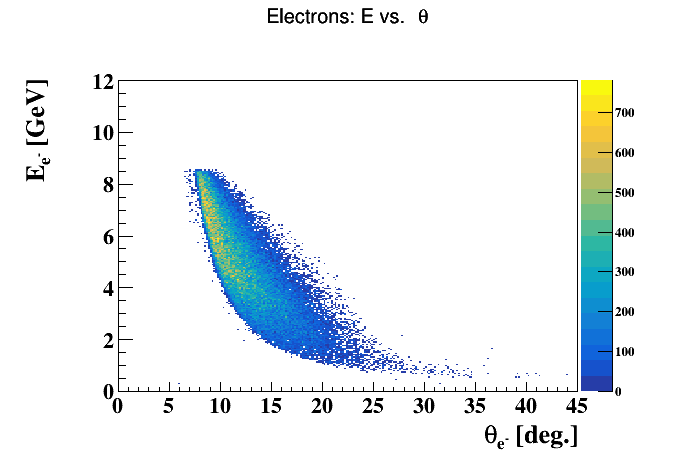
\includegraphics[width=0.48\textwidth,clip,trim=0mm 0mm 0mm 
   20mm]{figs/e_E_theta.png}
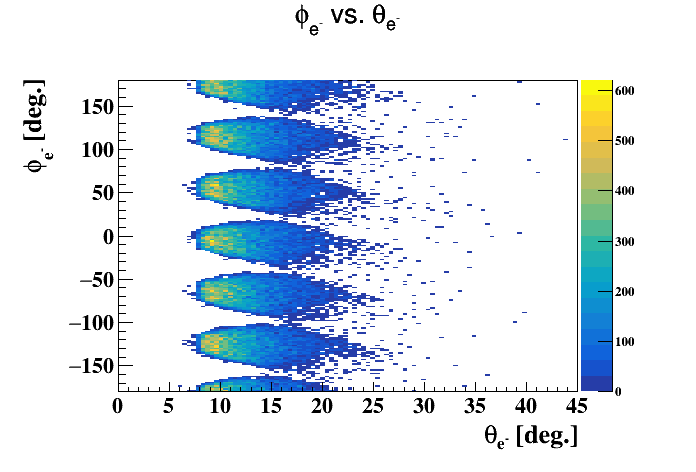
\includegraphics[width=0.48\textwidth,clip,trim=0mm 0mm 0mm 
   20mm]{figs/e_phi_theta.png}
   \caption{Electron's energy as a function of it's polar angle (left) and the 
   azimuthal angle as a function of the polar angle (right), for n-DVCS events.  
   Forward-CLAS12 acceptance and physics cuts are included.}
   \label{fig:el_kin}
\end{figure}
 
\begin{figure}[htb]
\centering
   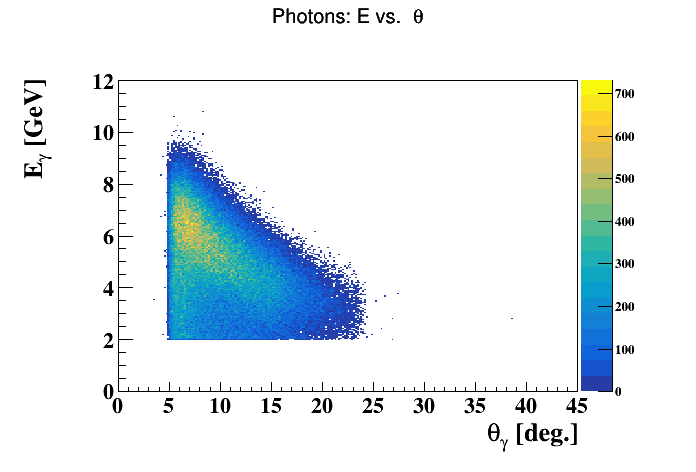
\includegraphics[width=0.48\textwidth,clip,trim=0mm 0mm 0mm 
   20mm]{figs/gamma_E_theta.png}
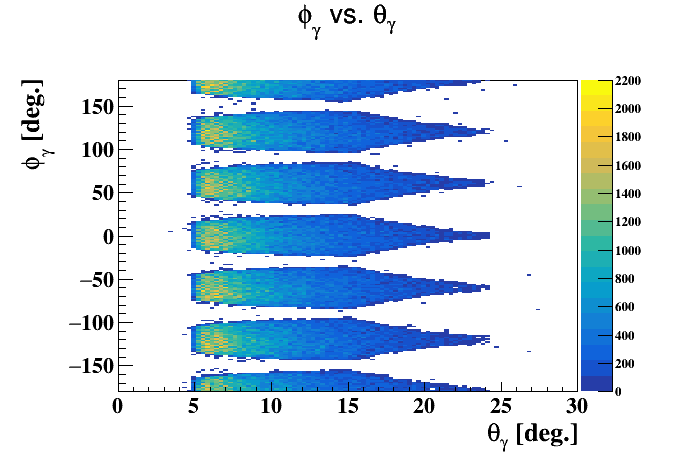
\includegraphics[width=0.48\textwidth,clip,trim=0mm 0mm 0mm 
   20mm]{figs/gamma_phi_theta.png}
   \caption{Photon's energy as a function of it's polar angle (left) and the 
   azimuthal angle as a function of the polar angle (right), for n-DVCS events.  
   Forward-CLAS12 acceptance and physics cuts are included.}
   \label{fig:photon_kin}
\end{figure}
 
\begin{figure}[htb]
\centering
   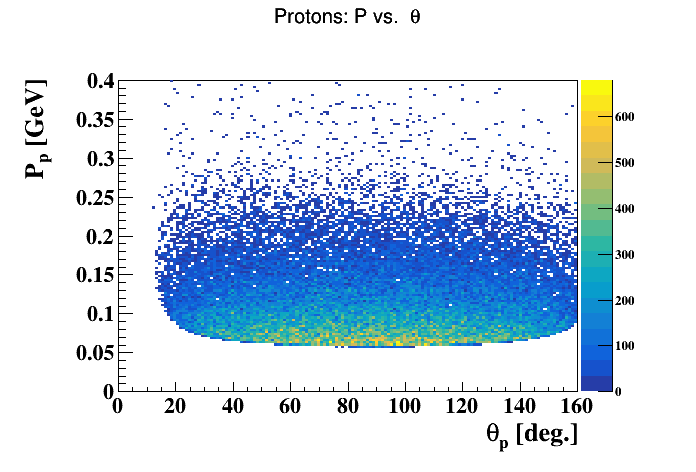
\includegraphics[width=0.48\textwidth,clip,trim=0mm 0mm 0mm 
   20mm]{figs/p_p_theta.png}
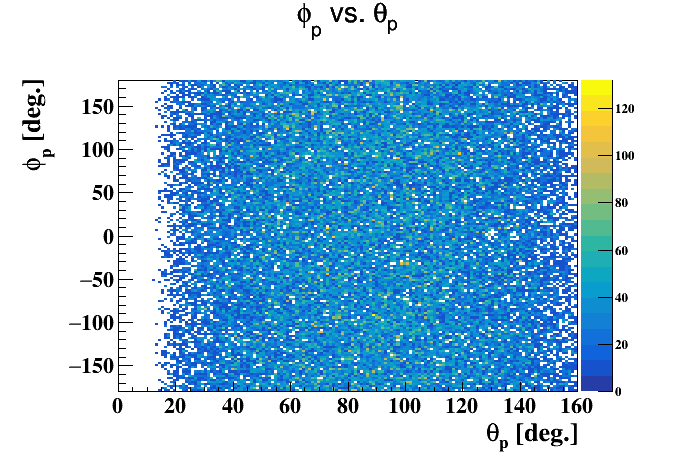
\includegraphics[width=0.48\textwidth,clip,trim=0mm 0mm 0mm 
   20mm]{figs/p_phi_theta.png}
   \caption{Recoiling proton's momentum as a function of it's polar angle 
   (left) and the azimuthal angle as a function of the polar angle (right), 
   from n-DVCS events. BONuS12 RTPC acceptance and physics cuts are included.}
   \label{fig:photon_kin}
\end{figure}
 
\begin{figure}[htb]
\centering
   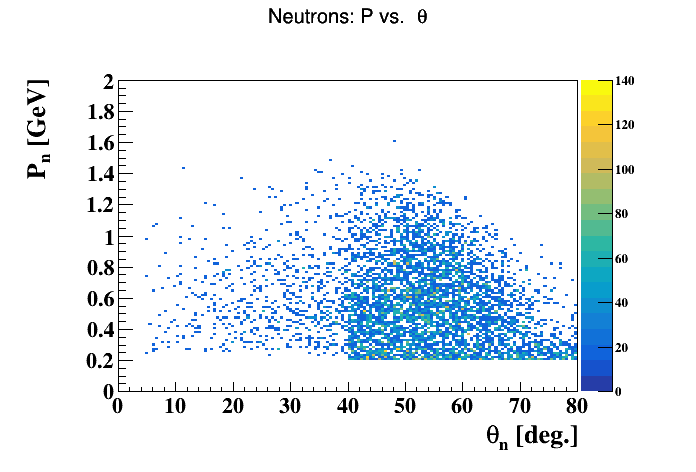
\includegraphics[width=0.48\textwidth,clip,trim=0mm 0mm 0mm 
   20mm]{figs/n_p_theta.png}
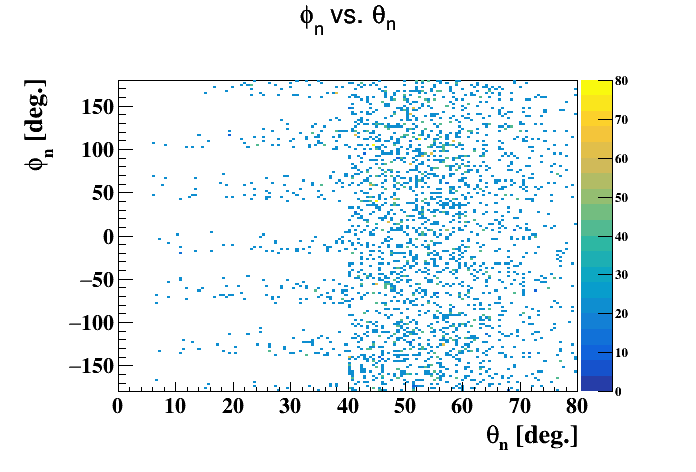
\includegraphics[width=0.48\textwidth,clip,trim=0mm 0mm 0mm 
   20mm]{figs/n_phi_theta.png}
   \caption{Recoiling neutron's momentum as a function of it's polar angle 
   (left) and the azimuthal angle as a function of the polar angle (right), 
   from n-DVCS events. BONuS12 RTPC acceptance and physics cuts are included.}
   \label{fig:photon_kin}
\end{figure}
 

\section{Projections}
\subsection{Semi-exclusive selection}


\begin{figure}[htb]
  \centering
    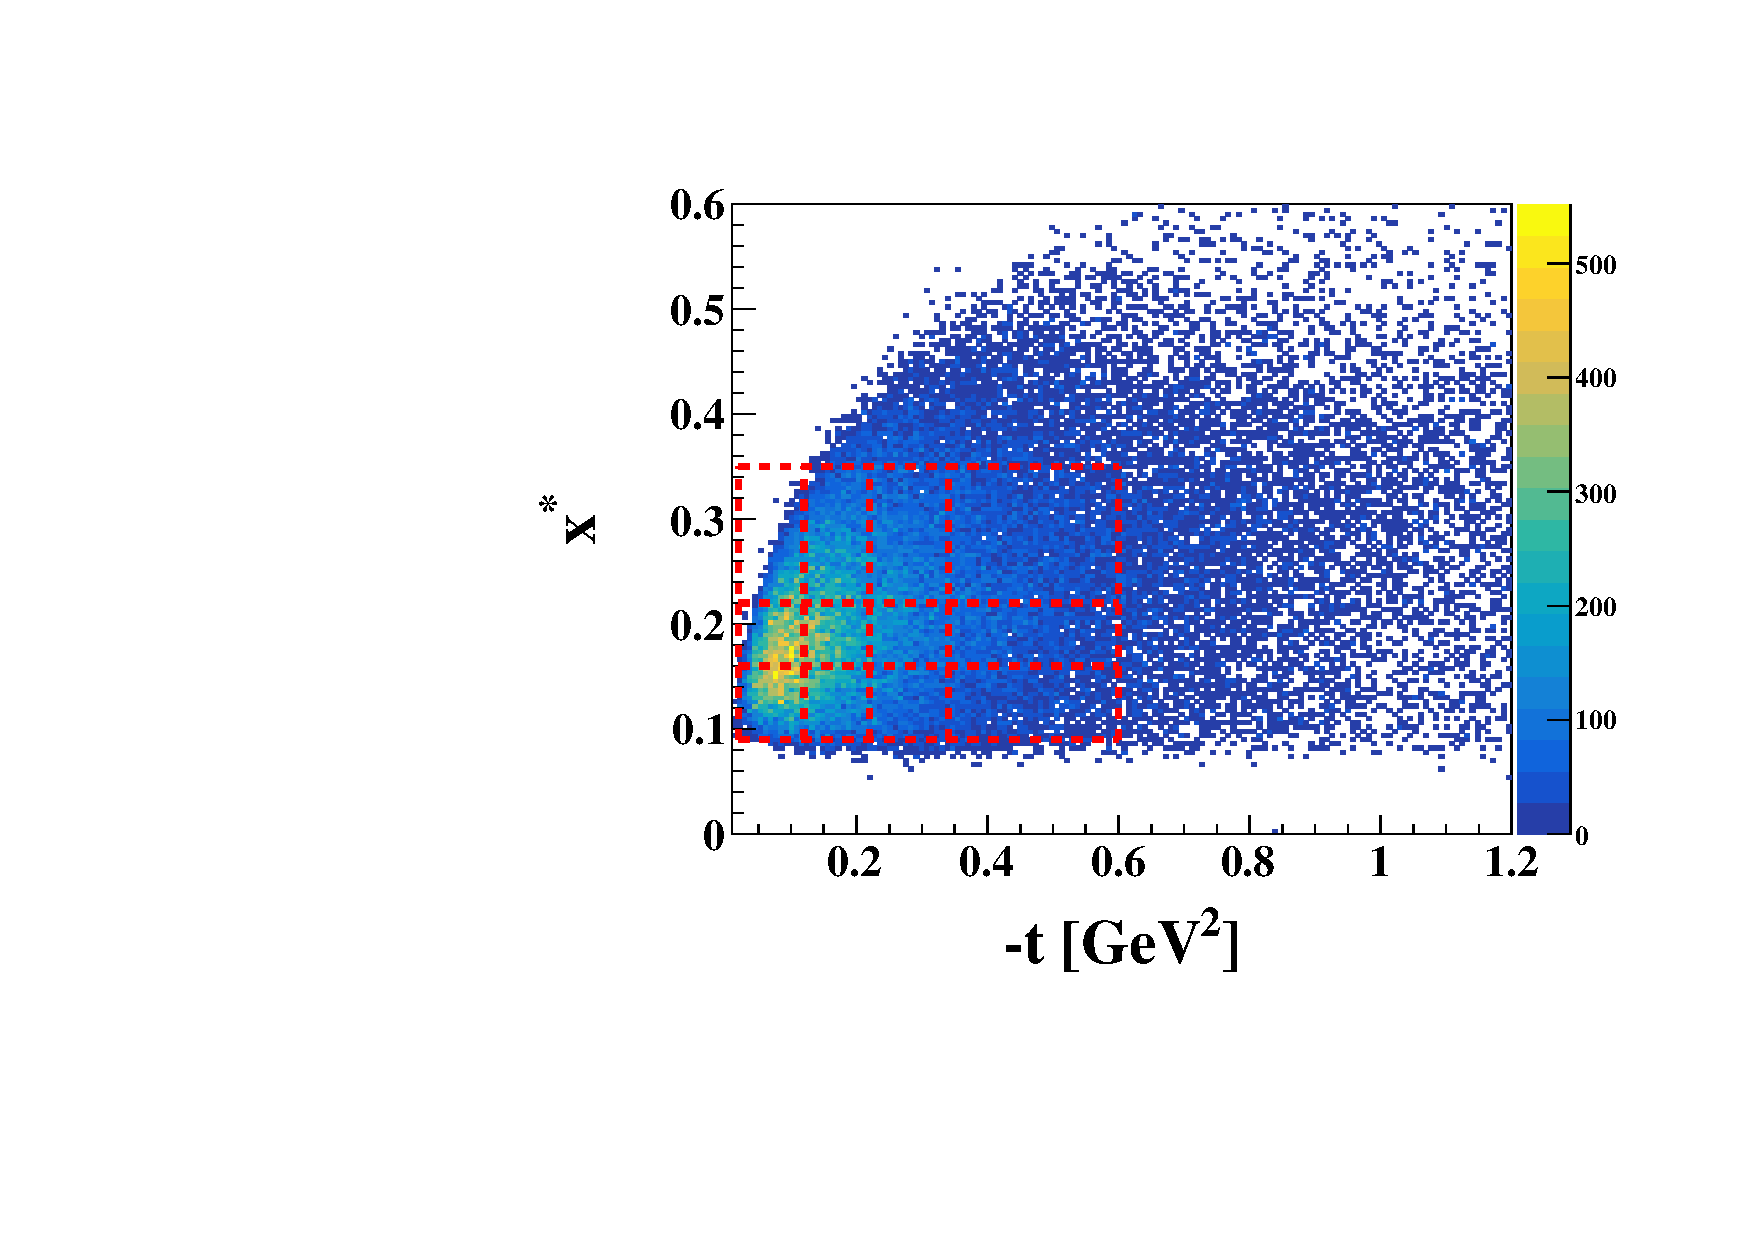
\includegraphics[width=0.55\textwidth,clip]{figs/pdf/t_x*.pdf}
  \caption{Data binning in $x^{*}$ vs $-t$ space.
   \label{fig:binning_x_t}}
\end{figure}

\begin{figure}[htb]
  \centering
    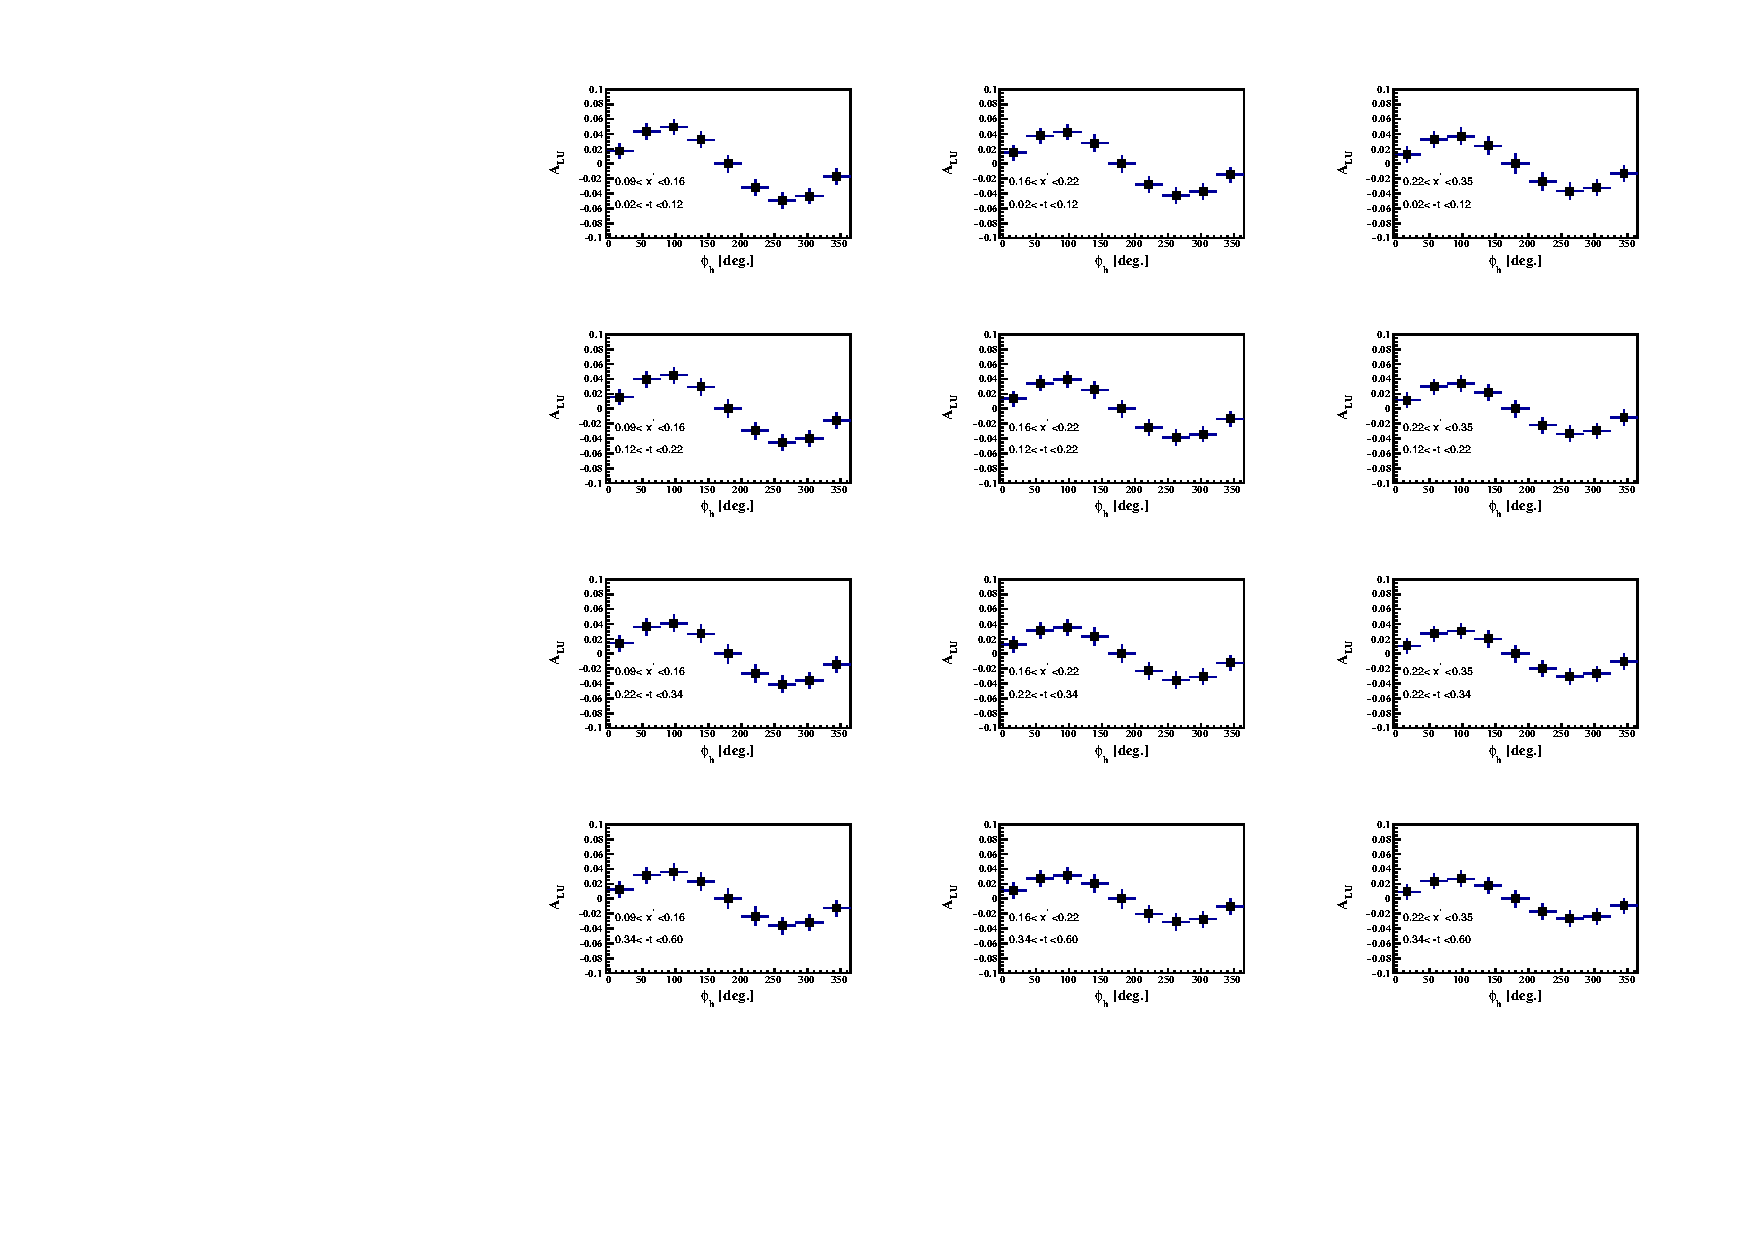
\includegraphics[width=1.1\textwidth,clip]{figs/pdf/BSA_incoherent_Phi_x_t.pdf}
  \caption{Projected beam-spin asymmetries as a function of the hadronic angle 
   $\phi_h$ in the binning of $x^{*}$ vs $-t$ space.
   \label{fig:alu_semi}}
\end{figure}




\subsection{Semi-exclusive selection}

\begin{figure}[htb]
  \centering
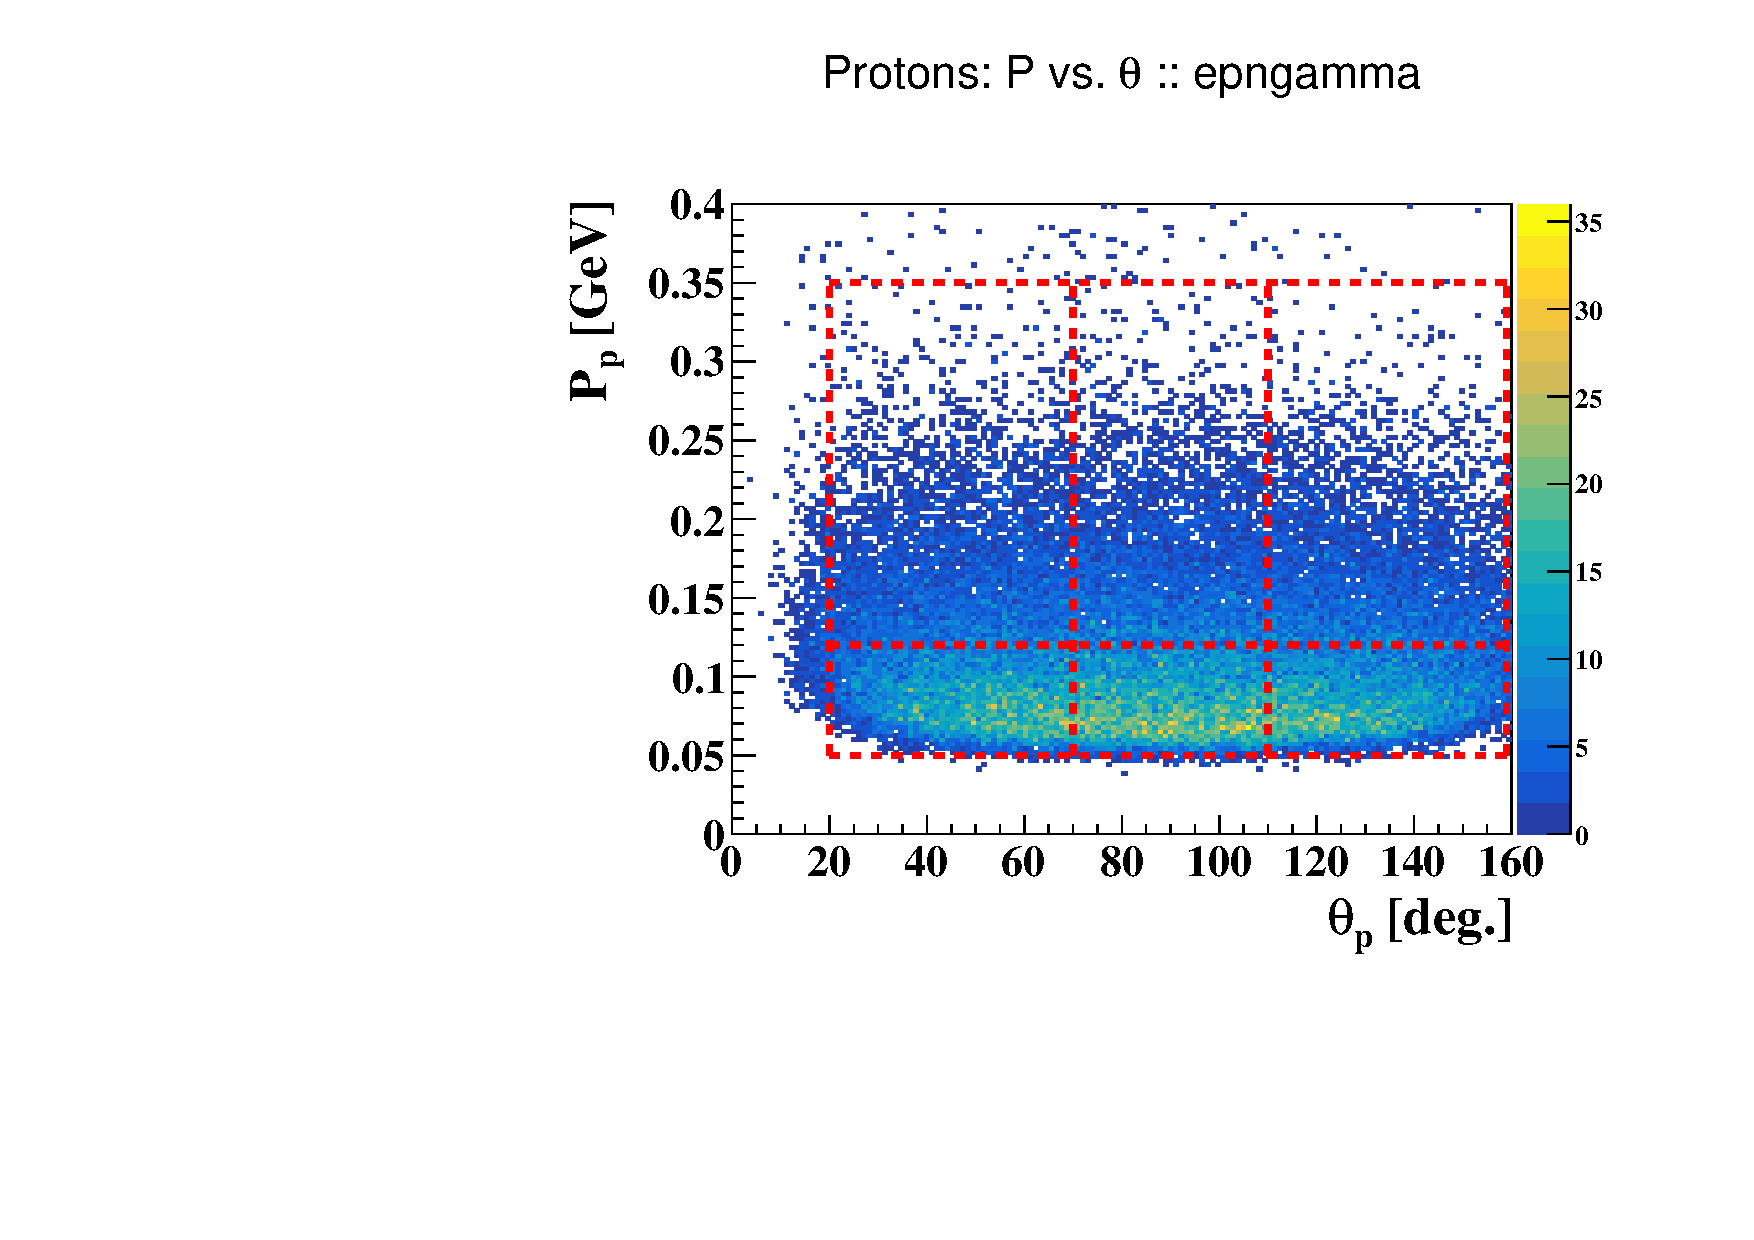
\includegraphics[width=0.55\textwidth,clip,trim=0mm 0mm 0mm 
   20mm]{figs_epngamma/pdf/epngamma_p_p_theta.pdf}
  \caption{Data binning in $p_s$ vs $\theta_s$ space.
   \label{fig:binning_x_t}}
\end{figure}

\begin{figure}[htb]
  \centering
    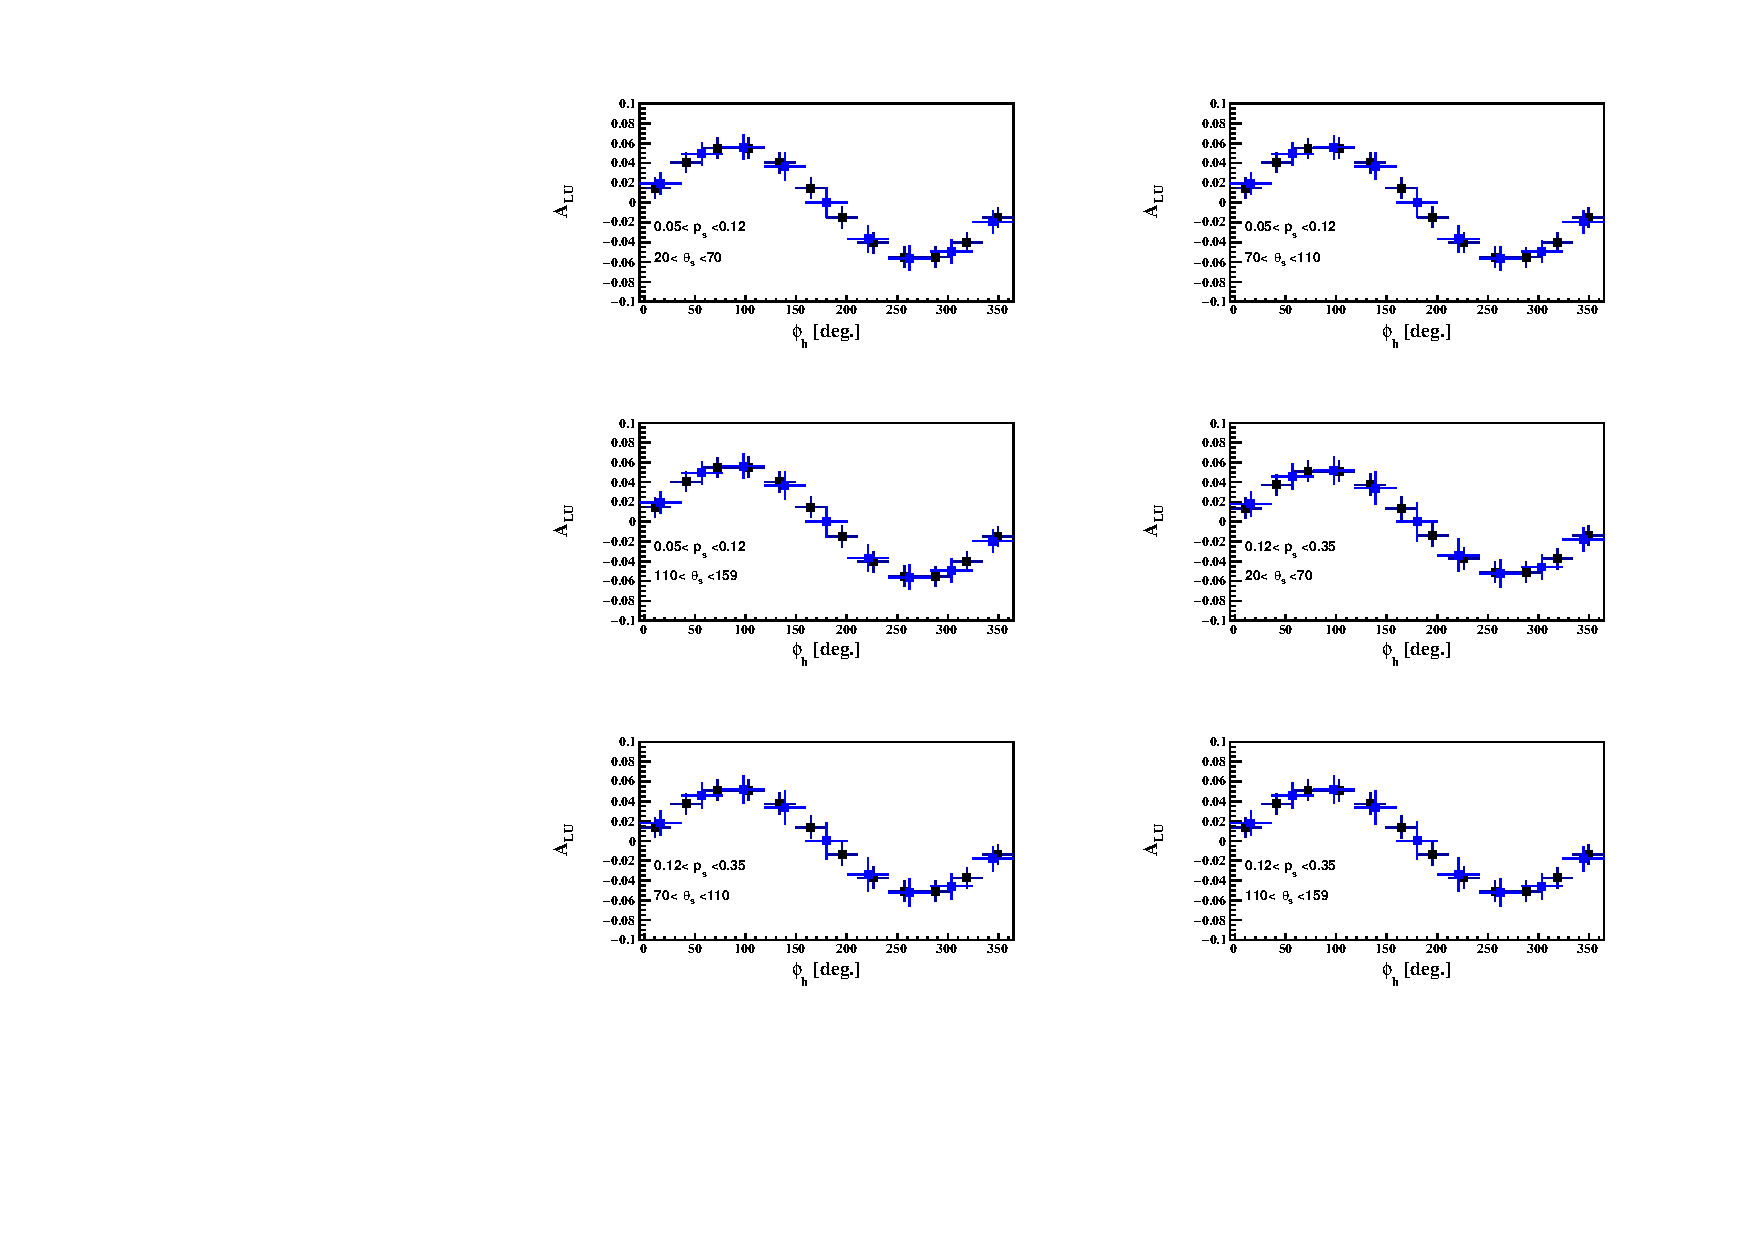
\includegraphics[width=1.1\textwidth,clip]{figs_epngamma/pdf/epngamma_BSA_incoherent_Phi.pdf}
  \caption{Projected beam-spin asymmetries as a function of the hadronic angle 
   $\phi_h$ in the binning of $p_s$ vs $\theta_s$ space.
   \label{fig:alu_semi}}
\end{figure}



